%!TEX root = main.tex
\section{Message passing systems}\label{sec:prelims}

%TODO A BUFFER FOR EVERY PAIR OF PROCESSES DOESN'T CHANGE THE RESULTS

We define a message passing system as the composition of a set of processes that exchange messages, which
can be stored in FIFO buffers before being received. An execution of such a system can be represented abstractly
using a partially-ordered set of events, called a \emph{trace}. The partial order in a trace represents, intuitively,
the causal relation between the events in an execution. We show that the systems we define satisfy a property
known as \emph{causal delivery} which states that the order in which messages are received by a process is
consistent with the causal relation between the corresponding sendings.

\subsection{Send and Receive Actions}

We fix arbitrary sets $\<Pids>$ and $\<Val>$ of process ids and message payloads. 
%A \emph{message} is a triple $m = \tup{i,j,p}$ where $i \in \<Ids>$ denotes the source, $j \in \<Ids>$ the destination, and $p \in \<Plds>$ the payload. 
%The set of messages is denoted by $\<Msgs>$. 
%The source, destination, and payload of a message $m$ are denoted by $\<src>(m)$, $\<dst>(m)$, $\<pay>(m)$, respectively.
%We fix an arbitrary set $\<Mids>$ of message identifiers, and the sets
For given sets $\<Ids>$ and $\<Plds>$, we fix the sets 
\begin{align*}
S = \set{\senda{p,q,v}: p,q\in\<Pids>, v\in \<Val>},\mbox{ and }R = \set{\reca{q,v}: q\in\<Pids>, v\in \<Val>}
\end{align*}
of \emph{send actions} and \emph{receive actions}. 
Each send action $\senda{p,q,v}$ combines two process ids $p, q\in \<Ids>$ denoting 
the sender and the receiver of the message, respectively, and a message payload $v\in \<Val>$. Receive actions
specify the process $q\in \<Pids>$ receiving the message, and the message payload $v\in \<Val>$. 
We write $\senda{p,q,\_}$ and $\reca{q,\_}$ when the message payload is unconstrained.
We denote the process executing a send/receive action $a\in S\cup R$ by $\<proc>(a)$, i.e.,
$\<proc>(a)=p$ for every $a=\senda{p,q,v}$, and $\<proc>(a)=q$ for every $a=\reca{q,v}$,
and the destination of a send action $s\in S$ by $\<dest>(s)$, i.e., $\<dest>(\senda{p,q,v})=q$.
The set of send, resp., receive, actions $a$ of process $p$, i.e., with $\<proc>(a)=p$, is denoted by $S_p$, resp., $R_p$.
%Send and receive actions $s\in S$ and $r\in R$ are \emph{matching}, written $s\match r$, when $\<msg>(s)=\<msg>(r)$.

\subsection{Message Passing Systems}

A message passing system consists of a finite set of processes that communicate via messages. Each process is described as a state
machine that evolves by executing send or receive actions.
%, and it is equipped with a FIFO buffer for storing incoming messages before being received. 
Local actions modifying the state of a process are omitted in order to simplify the technical exposition. 
%Also, extending our
%results to other types of buffers that don't satisfy the FIFO semantics are discussed in Section~\ref{}. 

%, or local actions (specified as $\epsilon$ transitions)
% and it is equipped with an instance of some fixed collection data type, e.g., FIFO queue, 
%that acts as a message buffer (storing incoming messages before being received). 

Formally, a \emph{message passing system} is a tuple $\mathcal{S}=((\<Lsts>_p,\delta_p,l_p^0)\mid p\in\<Pids>)$ 
%where each $S_p$ is a labeled transition system 
%$S_p=(\<Lsts>_p,\delta_p,l_p^0)$ 
where $\<Lsts>_p$ is the set of local states of process $p$,
$\delta_p\subseteq \<Lsts>\times (S_p\cup R_p)\times \<Lsts>$ is a transition relation describing the 
evolution of process $p$, and $l^0_p$ is the initial state of process $p$. Examples of message passing systems can be found in Figure~\ref{fig:commit}, Figure~\ref{fig:elevator}, and Figure~\ref{fig:replication}.

For a process $p$, a state $l\in \<Lsts>_p$ is called \emph{receiving} when $(l,a,l')\in\delta_p$, for some $l'$, implies that $a\in R_p$. For instance, the state {\tt Init} of the process {\tt Manager} in Figure~\ref{fig:commit} is receiving. The state $l$ is called \emph{final} when there exists no $l'$ and $a$ such that $(l,a,l')\in\delta_p$.

%, and $\<AdtM>$ is 
%a collection data type  with interface $\mathrm{add}(m)$ for adding an element $m$
%to the collection and $\mathrm{rem}()$ that removes and returns an element from the collection (this method returns only when the collection
%is non-empty, otherwise it blocks). 
%To simplify the exposition, we assume
%that each receive action is enabled in every local state, i.e., for every $l\in \<Lsts>$ and every $r\in R$, there exists $l'\in \<Lsts>$ such that $(l,r,l')\in \delta$.
%TODO GIVE MORE EXPLANATIONS

\subsection{Asynchronous Semantics}\label{ssec:semantics}

The semantics of a message passing system assumes that each process is equipped with a FIFO buffer for storing incoming messages, 
every send action enqueues the message into the destination's buffer, and every receive action dequeues a message from the corresponding 
buffer. Since messages are not received instantaneously, we use the term \emph{asynchronous} to refer to this semantics (to distinguish it
from a ``more synchronous'' semantics defined in Section~\ref{sec:criterion}). 

Formally, configuration $c=\tup{\vec{l},\vec{b}}$ is a vector  $\vec{l}$  of local states together with a vector $\vec{b}$ of message buffers  that are
represented as sequences of message payloads tagged with unique identifiers. The identifiers are used only for technical reasons, to identify a ``matching'' relation
between sends and receives.  These two vectors are indexed by elements of $\<Pids>$.
For a vector $\vec{x}$, let $\vec{x}_p$ denote the element of $\vec{x}$ of index $p$.
%The state of the process $p$ is defined by the local state $\vec{l}_p$ and the message buffer $\vec{b}_p$.
The initial configuration $c_0$ of the system $\mathcal{S}$ is the tuple of initial local states together with empty message buffers, i.e., 
$c_0=\tup{\vec{l},\vec{b}}$ where $\vec{l}_p=l_p^0$ and $\vec{b}=\epsilon$ for each $p\in\<Pids>$.
%The set of configurations is denoted by $C$.

\begin{figure} [t]
\footnotesize{
  \centering
  \begin{mathpar}
    \inferrule[send]{
      m= (i,v) \\ 
      i\in \<Mids>\mbox{ fresh} \\
      (\vec{l}_p,\senda{p,q,v},l)\in \delta_p 
    }{
      \vec{l},\vec{b}
      \xrightarrow{\send{i}{p,q,v}}
      \vec{l}[\vec{l}_p\gets l],\vec{b}[\vec{b}_q\gets \vec{b}_q\cdot m]
    }%\hspace{5mm}
    
    \inferrule[receive]{
      \vec{b}_q = (i,v) \cdot b \\
      (\vec{l}_q,\reca{q,v},l)\in \delta_q
    }{
      \vec{l},\vec{b}
      \xrightarrow{\rec{i}{q,v}}
      \vec{l}[\vec{l}_q\gets l],\vec{b}[\vec{b}_q\gets b]
    }%\hspace{5mm}
    
%    \inferrule[local]{ 
%      l\in \delta(\vec{l}_p,\epsilon) \neq \emptyset
%    }{
%      \vec{l},\vec{b}
%      \xrightarrow{\epsilon}
%      \vec{l}[\vec{l}_p\gets l],\vec{b}
%    }%\hspace{5mm}
  \end{mathpar}
  }
% \vspace{-5mm}
  \caption{The asynchronous semantics of a message passing system $\mathcal{S}$. For a vector $\vec{x}$, $\vec{x}[\vec{x}_p\gets E]$ is the vector $\vec{y}$ with $\vec{y}_q=\vec{x}_q$, for every $q\neq p$, and $\vec{x}_p=E$. Also, $\cdot$ denotes the concatenation of two sequences.
  %$\vec{b}[\vec{b}_q.\ \mathrm{add}(m)]$ denotes the vector of message buffers obtained from $\vec{b}$ by calling the method $\mathrm{add}(m)$ of the element of index $q$.
  }
  \label{fig:asynch-sem}
%\vspace{-6mm}
\end{figure}

We fix an arbitrary set $\<Mids>$ of message identifiers, and the sets 
\begin{align*}
S_{id} = \set{s_i: s\in S, i\in \<Mids>} \mbox{ and } R_{id} = \set{r_i: r\in R, i\in \<Mids>}
\end{align*}
of indexed actions; an indexed action combines a send/receive action with a message identifier $i\in \<Mids>$.
Message identifiers are used to pair send and receive actions.
We denote the message id of an indexed send/receive action $a$ by $\<msg>(a)$.
Indexed send and receive actions $s\in S_{id}$ and $r\in R_{id}$ are \emph{matching}, 
written $s\match r$, when $\<msg>(s)=\<msg>(r)$.
For notational convenience, we often associate $\<Mids>$ with $\<Nats>$, e.g., writing $\send{1}{p,q,v}$ and $\rec{2}{q',v'}$ in place of $\send{i_1}{p,q,v}$ and $\rec{i_2}{q',v'}$.

The transition relation $\rightarrow$ in Figure~\ref{fig:asynch-sem} is determined by a message passing system $\mathcal{S}$, and maps
a configuration $c_1$ to another configuration $c_2$ and indexed action $a\in S_{id}\cup R_{id}$.
The effect of a \textsc{send} transition is to enqueue the message payload tagged with a fresh identifier to the buffer of the destination, and the effect of a \textsc{receive} transition is to dequeue a message from the local buffer.

An \emph{execution} of a system $\mathcal{S}$ under the asynchronous semantics to configuration ${c}_n$
is a sequence of indexed actions $a_1 \ldots a_n$ such that 
there exists a configuration sequence ${c}_0 {c}_1 \ldots {c}_n$ with
%\vspace{-2mm}
%\begin{align*}
$  {c}_m \xrightarrow{a_{m+1}} {c}_{m+1}$
%\end{align*}
%%\vspace{-1.5mm}
%\noindent
for all $0 \le m < n$. 
We 
%call the sequence $a_1 \ldots a_n$ the \emph{log} of ${c}_0 {c}_1 \ldots
%{c}_n$ and we 
say that ${c}_n$ is reachable in $\mathcal{S}$ under the asynchronous semantics. % with log $a_1\ldots a_n$. 
The \emph{reachable local state vectors} of $\mathcal{S}$, denoted by $\asynchSt{\mathcal{S}}$, is the
set of local state vectors in reachable configurations.
%
The set of executions of $\mathcal{S}$ under the asynchronous semantics is denoted by $\asynchExec{\mathcal{S}}$.
In the following, we don't distinguish between executions obtained by a consistent renaming of the message identifiers. 

Given an execution $e$, a send action $s$ in $e$ is called an \emph{unmatched send} when $e$ contains no receive action $r$ such that $s\match r$. An execution $e$ is called \emph{matched} when it contains no unmatched send.

\subsection{Traces}

%TODO SEE ABOUT THIS EQUALITY UP TO SUBSTITUTIONS OF MESSAGE IDENTIFIERS

Executions are represented abstractly using traces which are sets of indexed actions together with a \emph{program order} relation relating every two actions of the same process and a \emph{source} relation relating a send with the matching receive (if any).

A trace is a tuple $t=(A,po,src)$ where $A\subseteq S_{id}\cup R_{id}$, $po\subseteq A^2$ defines a total order between actions executed by the same process, i.e., for every $p\in\<Pids>$, $po\cap \{a: a\in A\mbox{ and }\<proc>(a)=p\}^2$ is a total order, and $src\subseteq S_{id}\times R_{id}$ is a relation such that $src(a,a')$ iff $a\match a'$.
The \emph{trace} of an execution $e$, denoted by $tr(e)$, is the tuple $(A,po,src)$ where $A$ is the set of all actions in $e$, $po(a,a')$ iff $\<proc>(a)=\<proc>(a')$ and $a$ occurs before $a'$ in $e$, and $src(a,a')$ iff $a\match a'$. Examples of traces can be found in Figure~\ref{fig:commit-exec}, Figure~\ref{fig:elevator-exec}, Figure~\ref{fig:replic-exec}.
%

\begin{proposition}
For a trace $t=(A,po,src)$, the union of $po$ and $src$ is acyclic.
\end{proposition}

Let $\asynchTr{\mathcal{S}}=\set{tr(e):e\in \asynchExec{\mathcal{S}}}$ be the set of traces of $\mathcal{S}$ under the asynchronous semantics.

Traces abstract away the order between actions that are not ``causally'' related, e.g., two send actions of two different processes that could be executed in any order. 
%Reordering actions which are not causally related in an execution leads to another execution that 
%We define a conflict relation $\prec$ on actions in $S_{id}\cup R_{id}$ that relates every two actions of the same process and every send with the matching receive. Formally,
%\begin{align*}
%a \prec a'\mbox{ iff } \<proc>(a) = \<proc>(a')\mbox{ or } a\match a'
%\end{align*}
%
Two executions have the same trace when they only differ in the order between such actions.
Formally, given an execution $e=e_1\cdot a\cdot a'\cdot e_2$ with $tr(e)=(A,po,src)$, where $e_1, e_2\in (S_{id}\cup R_{id})^*$ and $a,a'\in S_{id}\cup R_{id}$, we say that the execution $e'=e_1\cdot a'\cdot a\cdot e_2$ is derived from $e$ by a \emph{valid swap} iff $(a,a')\not\in po\cup src$. A permutation $e'$ of an execution $e$ is \emph{conflict-preserving} when $e'$ can be derived from $e$ through a sequence of valid swaps. 
From now on, whenever we use the term permutation we mean conflict-preserving permutation.

\begin{example}\label{ex:perm}
The following traces 
\begin{align*}
\send{1}{p_1,q,\_}\ 
\send{2}{p_2,q,\_}\ 
\rec{1}{q,\_}\ 
\rec{2}{q,\_} \\
\send{1}{p_1,q_1,\_}\ 
\send{2}{p_2,q_2,\_}\ 
\rec{2}{q_2,\_}\ 
\rec{1}{q_1,\_} 
\end{align*}
have the following conflict-preserving permutations, respectively:
\begin{align*}
\send{1}{p_1,q_1,\_}\ 
\rec{1}{q,\_}\ 
\send{2}{p_2,q,\_}\ 
\rec{2}{q,\_} \\
\send{1}{p_1,q_1,\_}\ 
\rec{1}{q_1,\_}\ 
\send{2}{p_2,q_2,\_}\ 
\rec{2}{q_2,\_}\ 
\end{align*}
\end{example}

A direct consequence of the definitions is that the set of executions having the same trace are permutations of one another. 

\begin{lemma}
Let $e$ be an execution. Then, for every execution $e'$ such that $tr(e)=tr(e')$, we have that $e'$ is a permutation of $e$ or vice-versa. % (modulo a substitution of message identifiers).
%and $e_2$ be  two executions such that $tr(e_1)=tr(e_2)$. Then, $e_1$ is a permutation of $e_2$ or vice-versa (modulo a substitution of message identifiers).
\end{lemma}

%A message passing system can not distinguish between two executions, one being a conflict-preserving permutation of the other.


The following lemma shows that a message passing system $\mathcal{S}$ cannot distinguish between permutations or equivalently, executions having the same trace.
%admits an execution $e'$ whenever it admits an execution $e$ with $tr(e)=tr(e')$.

\begin{lemma}\label{lem:undist}
If $e'$ is a permutation of an execution $e\in \asynchExec{\mathcal{S}}$ to configuration $c_n$, then $e'$ is also an execution of $\mathcal{S}$ to configuration $c_n$.
Also, if $e\in \asynchExec{\mathcal{S}}$, then $e' \in \asynchExec{\mathcal{S}}$ for every execution $e'$ such that $tr(e)=tr(e')$.
\end{lemma}

\subsection{Causal Delivery}

The asynchronous semantics ensures a property known as \emph{causal delivery}, which intuitively, says that the order in which messages are received by a process $q$ is consistent with the ``causal'' relation between them. Two messages are causally related if for instance, they were sent by the same process $p$ or one of the messages was sent by a process $p$ after the other one was received by the same process $p$. This property is ensured by the fact that the message buffers have a FIFO semantics and a sent message is instantaneously enqueued in the destination's buffer. For instance, the trace (execution) on the left of Figure~\ref{fig:ex-causal-delivery} satisfies causal delivery. In particular, the messages $v1$ and $v3$ are causally related, and they are received in the same order by $q2$. On the other hand, on the right of Figure~\ref{fig:ex-causal-delivery}, we give a trace where the messages $v_1$ and $v_3$ are causally related, but received in a different order by $q2$, which implies that the trace doesn't satisfy causal delivery. This trace is not admitted by the asynchronous semantics defined in Section~\ref{ssec:semantics} because the message $v1$ would be enqueued in the buffer of $q2$ before $\senda{p,q1,v2}$ is executed and thus, before $\senda{q1,q2,v3}$ as well.

\begin{figure}[t]
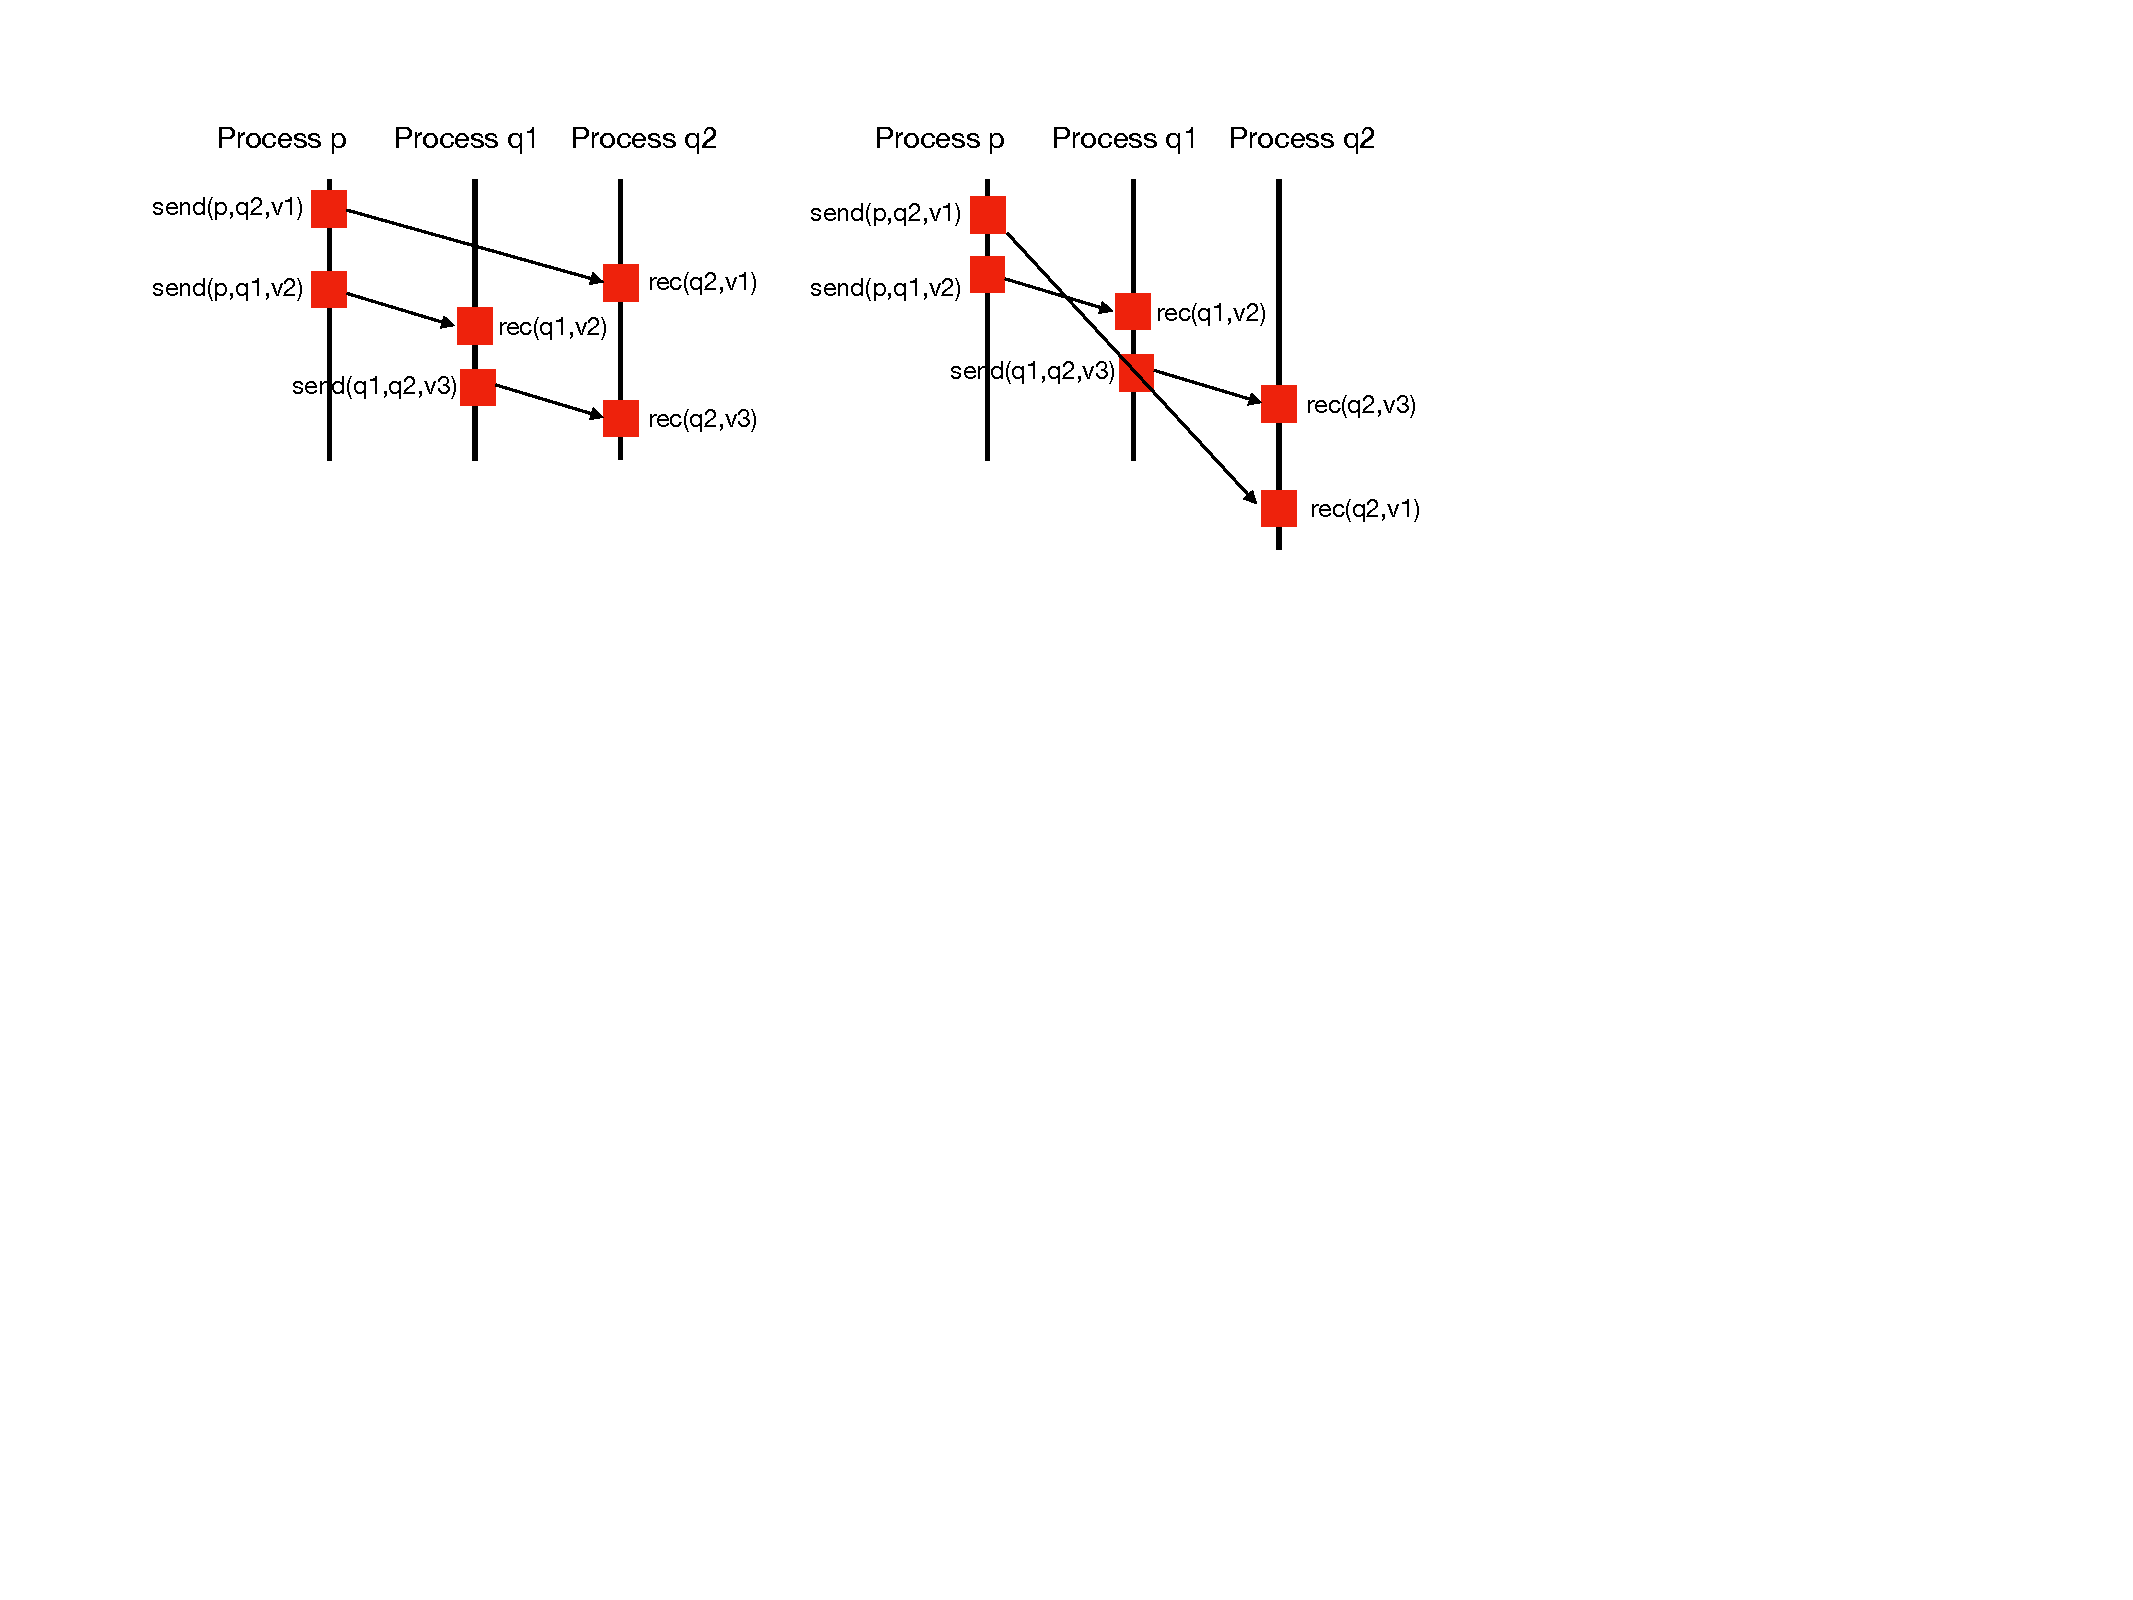
\includegraphics[width=9cm]{ex-causal-delivery.pdf}
\caption{A trace satisfying causal delivery (on the left) and a trace violating causal delivery (on the right).}
\label{fig:ex-causal-delivery}
\end{figure}

Formally, for a trace $t=(A,po,src)$, the transitive closure of $po\cup src$, denoted by $\leadsto_t$, is called the \emph{causal relation} of $t$. For instance, for the trace $t$ on the left of Figure~\ref{fig:ex-causal-delivery}, we have that $\senda{p,q2,v1}\leadsto_t \senda{q1,q2,v3}$.
A trace $t$ satisfies \emph{causal delivery} if the order between receive actions executed by the same process $p$ is consistent with the causal relation between send actions with destination $p$, i.e., for every two send actions $s_1$ and $s_2$ in $A$, 
\begin{align*}
(s_1\leadsto_{t} s_2\land \<dest>(s_1)=\<dest>(s_2))\implies (\not\exists r_2\in A.\ s_2\match r_2)\lor (\exists r_1,r_2\in A.\ s_1\match r_1\land s_2\match r_2\land (r_2,r_1)\not\in po)
\end{align*}

An execution $e$ satisfies causal delivery when the trace $tr(e)$ satisfies causal delivery.

\begin{lemma}
Every trace $t\in \asynchTr{\mathcal{S}}$ satisfies causal delivery. 
\end{lemma}

